\documentclass[notitlepage]{article}
\usepackage[margin=0.75in]{geometry}
\usepackage{graphicx}
\author{Chris Manchester, Orren Saltzman}
\title{CIS 573 Project: Runtime Metamorphic Testing with Calico}
\parindent 0pt
\parskip 10pt

\begin{document}
\maketitle

\section{Introduction}

Calico is a C source code translator and annotation language used to perform runtime metamorphic property testing of C programs. Calico takes a C source file as input in which one or more functions has been annotated by the user according to an annotation language used to specify metamorphic properties. Calico's output is a C program that behaves exactly as the original, except that each time an annotated function is called, it is called again with transformed inputs, and the result is recorded. The original output is also transformed, and it is asserted by the new program that the two results are equal. If they are, nothing has been demonstrated about the correctness of the program, but if they are not, then a metamorphic property asserted by the user has been violated, and the function under test has been to shown to contain a fault.

\begin{figure}[ht!]
\centering
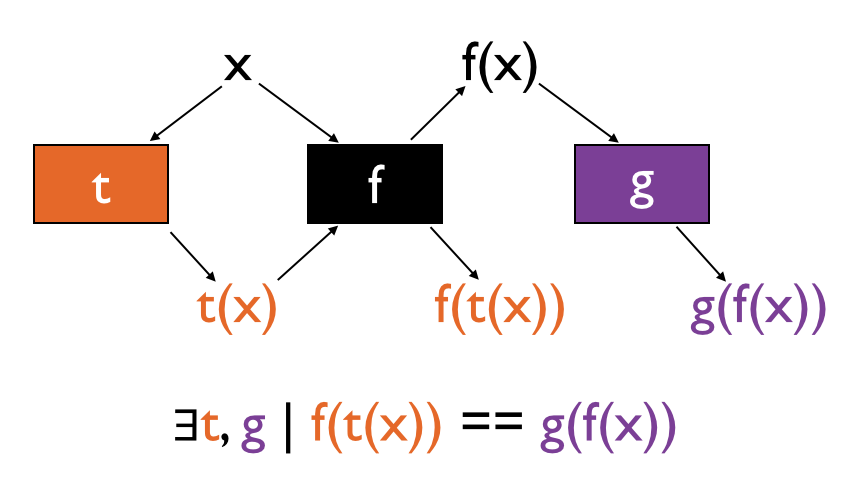
\includegraphics[width=175mm]{calico_pic1_alternate.png}
\caption{To specify a metamorphic property for the Function Under Test, f, the user must specify some functions t and g such that this equality holds.}
\end{figure}

\section{A Brief Description of Calico Instrumentation}

Many functions use side effects to accomplish their task. Furthermore, the data that might constitute the ``result'' of a C function is not necessarily the same as the return value of that function. It is therefore necessary to assume that any piece of memory belonging to the process of the program might be considered for the purpose of these assertions. It is necessary to sandbox the effects of the function under test each time it is called by spawning a new process for each property asserted. For instance, if a function is called by the application 100 times over the course of program execution, and three properties about the function are specified, then the instrumented program must make 400 calls to the function: The original 100, plus 100 for each specified input transformation. For each of the 300 transformed calls, a process must be spawned and the result recovered by the main process through the use of shared memory.

The form of the instrumented application is as follows:

\begin{figure}[ht!]
\centering
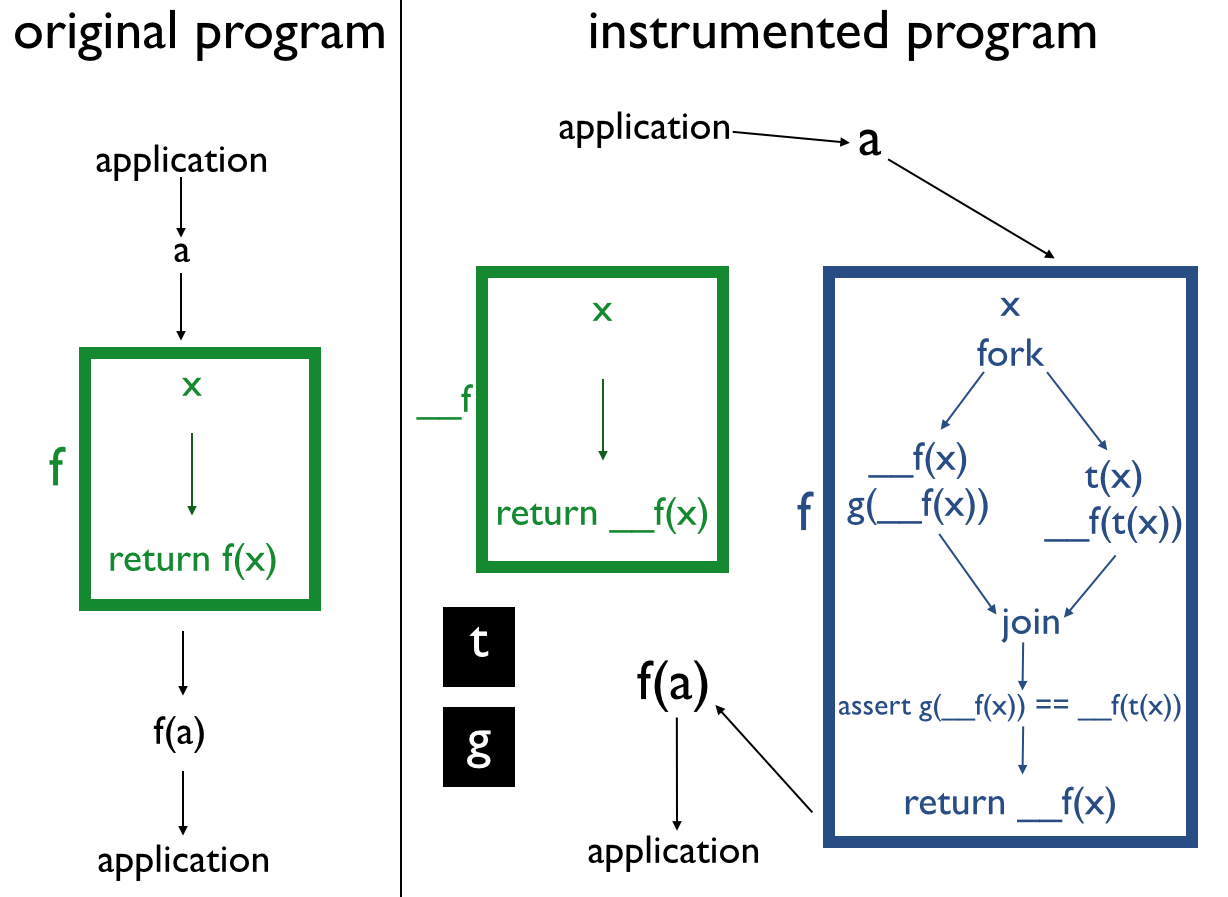
\includegraphics[width=175mm]{calico_pic2.png}
\caption{Calls to the function f are intercepted by a new function of the same name. The original is renamed with two leading underscores.}
\end{figure}

\section{The Annotation Language}

Annotations are written in C comments directly preceding the function under test.

A function annotation starts with a section containing information about the return type of the function under test, the return type of each parameter, and the identifiers associated with the function and each of its parameters. Metamorphic properties are then specified by one or more sets of property annotations. A property annotation set consists of an input property to transform each input, an output property to transform the output of the function, and two optional annotations. The optional state recovery annotation is used to specify a pointer to memory that is to be considered the result of the function, while the optional equality annotation will be used in these cases if a notion of equality other than bitwise equality (implemented with memcmp) should be used to compare the original and transformed outputs.

A more formal description of the annotation language is given by the following grammar. Non-terminals are enclosed by angle braces. All other symbols compose terminals in the grammar. The non-terminal ``string-literal'' corresponds to any sequence of characters enclosed by quotations, while the non-terminal ``C-identifier'' corresponds to identifiers specified by the C language.

\ttfamily

<annotated-comment> ::= <function-info-annotation> <param-annotations> <property-sets> \\

<function-info-annotation> ::= @fun-info \{ <function-name>, <type> \} ; \\

<param-annotations> ::= <param-annotation> \\
\phantom{1}\hspace{105pt}| <param-annotation> <param-annotations> \\

<param-annotation> ::= @param-info \{ <C-identifier>, <type> \} ; \\

<property-sets> ::= <property-set> \\
\phantom{1}\hspace{85pt}| <property-set> <property-sets> \\

<property-set> ::= <input-property> <output-property> \\
\phantom{1}\hspace{82pt}| <input-property> <output-property> <state-recovery> \\
\phantom{1}\hspace{82pt}| <input-property> <output-property> <state-recovery> <equality> \\

<input-property> ::= @input-prop \{ <property-list> \} ; \\

<property-list> ::= <property-elem> \\
\phantom{1}\hspace{85pt}| <property-elem>, <property-list> \\

<output-property> ::= @output-prop \{ <property-elem> \} ; \\

<state-recovery> ::= @state-recover \{ <property-elem>, <property-elem>, <property-elem> \} ;

<equality> ::= @equality-op \{ <property-elem> \} ;

<property-elem> ::= <C-identifier> \\
\phantom{1}\hspace{85pt}| <string-literal> \\

<type> ::= <string-literal>


\rmfamily

\section{A short example: summing an array}

The following file (sum\_example.c) contains a function, sum, and a stub main function which calls sum on a small array and prints the result:

\begin{verbatim}
#include <stdio.h>

extern void exit(int);

/**
 * May sum the elements of an array
 *
 * @fun-info { sum, "int" } ;
 * @param-info { arr, "int*" } ;
 * @param-info { length, "int" } ;
 * @input-prop { multiply_int_array(arr, 2, length), id } ;
 * @output-prop { double_int(result) } ;
 * @input-prop { duplicate(arr, length), double_int(length) } ;
 * @output-prop { double_int(result) } ;
 */
int sum ( int arr [], int length ) {
  int i = 0, r = 0;
  for (; i < length;) r += arr[i++];
  return r;
}

int main () {
  int arr [] = {1, 2, 3};
  int x = sum(arr, 3);
  printf("*** The sum is : %d\n", x);
  exit(0);
}
\end{verbatim}

The sum function has been annotated to assert two of its metamorphic properties. The first is that if each element of the input array is doubled, the resulting output should also be doubled. The second is that if the original array is replaced with one of twice its length consisting of the original array end to end, the result should be double.

Instrumentation by calico results in the following file (calico\_gen\_sum\_example.c):

\begin{verbatim}
#include "calico_prop_library.h"
#include <stdio.h>

extern void exit(int);


/**
 * May sum the elements of an array
 *
 * @fun-info { sum, "int" } ;
 * @param-info { arr, "int*" } ;
 * @param-info { length, "int" } ;
 * @input-prop { multiply_int_array(arr, 2, length), id } ;
 * @output-prop { double_int(result) } ;
 * @input-prop { duplicate(arr, length), double_int(length) } ;
 * @output-prop { double_int(result) } ;
 */

int __sum( int arr [], int length ) {
  int i = 0, r = 0;
  for (; i < length;) r += arr[i++];
  return r;
}

int sum( int arr [], int length )  {
    int numProps = 2;
    size_t result_sizes[numProps];
    int* shmids = malloc(numProps * sizeof(int));
    int procNum = -1;
    int i;
    int *orig_result = malloc(sizeof(int));
    result_sizes[0] = sizeof(int);
    int* t_result0 = NULL;
    int* g_result0 = malloc(result_sizes[0]);

    result_sizes[1] = sizeof(int);
    int* t_result1 = NULL;
    int* g_result1 = malloc(result_sizes[1]);

    for (i = 0; i < numProps; i += 1) {
        if (procNum == -1) {
            if ((shmids[i] = shmget(key++, result_sizes[i], IPC_CREAT | 0666)) < 0) {
                perror("shmget");
                exit(1);
            }
            if (0 == fork()) {
                procNum = i;
                break;
            }
        }
    }

    if (procNum == -1) {
        *orig_result = __sum(arr, length);
        for (i = 0; i < numProps; i += 1) {
            wait(NULL);
        }
    }

    if (procNum == 0) {
        t_result0 = shmat(shmids[0], NULL, 0);
// < input_transformation
        multiply_int_array(arr, 2, length);
// input_transformation >;
        // < input_transformation
        ;
// input_transformation >// < call_inner_function
        *t_result0 = __sum(arr, length);
// call_inner_function >
        shmdt(t_result0);
        exit(0);
    }

    if (procNum == 1) {
        t_result1 = shmat(shmids[1], NULL, 0);
// < input_transformation
        arr = duplicate(arr, length);
// input_transformation >;
// < input_transformation
        length = double_int(length);
// input_transformation >// < call_inner_function
        *t_result1 = __sum(arr, length);
// call_inner_function >
        shmdt(t_result1);
        exit(0);
    }

    t_result0 = shmat(shmids[0], NULL, 0);
// < output_transformation
    *g_result0 = double_int(*orig_result);
// output_transformation >
    if (memcmp(g_result0, t_result0, sizeof(int))) {
        printf("a property has been violated:\ninput_prop: multiply_int_array, id\noutput_prop: double_int(result)\n");

    }

    t_result1 = shmat(shmids[1], NULL, 0);
// < output_transformation
    *g_result1 = double_int(*orig_result);
// output_transformation >
    if (memcmp(g_result1, t_result1, sizeof(int))) {
        printf("a property has been violated:\ninput_prop: duplicate, double_int\noutput_prop: double_int(result)\n");

    }

    free(shmids);
    return *orig_result;
}


int main () {
  int arr [] = {1, 2, 3};
  int x = sum(arr, 3);
  printf("*** The sum is : %d\n", x);
  exit(0);
}
\end{verbatim}

\section{Known Limitations/Future Work}

\subsection{probabilistic testing}

Instrumenting an application causes its runtime to increase, primarily due to the overhead of spawning new processes (The specific runtime costs associated with instrumentation are described in the next section). One feature that would allow the user to mitigate this would be to optionally accept a probability parameter through the annotation language. This probability, set to 1 by default, would determine the likelihood of a test being run each time a function under test is called by the application. In this way, the probability parameter can be fine-tuned such that performance comes back within whatever range is considered acceptable to the user. Because of the element of randomness in such a feature, a bias in which certain kinds of inputs from the application are under-represented during testing would be unlikely, even though fewer total tests would be run.

\subsection{more sophisticated parsing methods}

The current implementation of the annotation parser requires information about the function under test and each of its parameters to be specified in the annotation language. This information must correspond to the source exactly, and duplicates the information in the function header. To reduce the user's burden while annotating the function and mitigate errors due to mis-annotation, the parser could instead parse the declarations in the function header to determine the required names and types of the function and parameters directly.

\subsection{optimizations in memory management}

Calico will not optimally instrument a certain subset of C functions with respect to memory management. Notably, functions which perform side effects on large regions of memory will create redundant copies of those regions in the instrumented version of the function. Changes could be made to calico's source translator that cause it to identify situations where copying memory is not necessary and direct reads of data to an original location rather than a location containing a copy.

Benefits of this feature in terms of space complexity would be linear with respect to the size of the inputs and outputs of the function under test. Benefits in terms of runtime complexity would be the similar, however the overhead of process spawning and deallocation is expected to be more expensive than these calls to memcpy, and significant runtime gains should not be expected.

\section{Performance Measurement}

An experiment was run using a Machine Learning application called Martirank. Martirank contains an implementation of merge sort which takes as input the location of an array, and type and size information about the elements of that array. It then sorts the array in place.

This function was annotated to assert the following metamorphic property: If the elements of the input array are permuted, the resulting array should be the same. Note that because the array is sorted in-place, the ``result'' as we are choosing to think about it now is not the same as the return value of the function. This is handled with the optional state recovery and equality annotations described earlier.

Martirank was run and timed with an example dataset. An instrumented version was created and timed using the same dataset, and the following results were observed:

\begin{tabular}{l | l | l}
& original & instrumented \\ \hline
calls to mergesort & $11047$ & $22094$ \\
total runtime (sec) & $.559$ & $24.403$ \\
new processes spawned & 0 & $11047$
\end{tabular}

Our resultant estimation of added runtime per assertion is $\frac{24.403}{11047} = {\mathbf .0022}$ seconds.

Note that the original runtime was not subtracted from the total, since the experiment was run on a multi-core machine that parallelized the new calls with the old. Thus, the new calls are assumed to represent the main runtime bottleneck of the program.

\section{Calico's Implementation}

Calico is implemented in OCaml, a functional language well-suited to the task of source code rewriting. It consists of two main modules, calico/parser, which handles the annotated C source inputs and parses them into data structures, and calico/writer, which takes the parsed annotation structure and writes a new C source file.

\subsection{Description of the Parser}

The Parser consists of a series of transformations based on an annotated C source. First, the source file is parsed into sections of C source and comments (those indicated with ``/*'' and ``*/''). The resulting list of program elements is traversed and inspected for the presence of annotated functions. If an annotated comment is detected (by the presence of a function info annotation in the comment text), the parser attempts to parse the comment according to the annotation language and if successful replaces this comment/source pair in the list of program elements with an annotated function data structure composed of information about the function and its annotations, the original function header, and the original function body. If no errors are encountered, the resulting list of program elements and function annotations are output for use by the source translator.

\subsection{Description of the Source Translator}

The writer module has one primary file, calico\_writer.ml, which takes as input the data structure defined in ast.ml and proceeds to create an instrumented C source program with the same file path as the original, but with ``calico\_gen\_'' affixed to the beginning of the file name.

\end{document}
